\section{Experiments}
\label{sec:exp}

We compare color-mapping immunization with eleven additive defenses. After the setup in \cref{sec:exp_setup}, \cref{sec:exp_anti} reports the main result, the edit displacement that remains after purification at matched distortion. \Cref{sec:exp_plane} places all defenses on the distortion--displacement plane before purification and lists their native budgets, and \cref{sec:exp_purify} measures how much of each perturbation purification removes. We then evaluate other editors in \cref{sec:exp_gen} and the perceptual quality of the protected images in \cref{sec:exp_percept}, and conclude with ablations in \cref{sec:exp_ablation}.

\subsection{Setup}
\label{sec:exp_setup}
\paragraph{Data.} Eight $512^2$ portraits with subject masks. \TODO{Portraits from Pexels, $N = 306$ to $500$.}
\paragraph{Attack.} InstructPix2Pix~\cite{brooks2023instructpix2pix} with Euler-Ancestral sampling (50 steps, text guidance 7.5, image guidance 1.8, seed 20260812) and the four accessory instructions of FaceLock~\cite{wang2025facelock}, giving $8 \times 4 = 32$ edits per method.
\paragraph{Purification.} Seven standard operations: JPEG at quality 80, 50, and 30; Gaussian blur with $\sigma = 1$ and $2$; a 10\% crop followed by resizing; and a $15^\circ$ rotation. VAE-Trans~\cite{purifyonce2026}, a fine-tuned VAE encoder used as a purifier, is reported separately.
\paragraph{Baselines.} Eleven additive methods. Each is rescaled to a common defense LPIPS (the matched-distortion arm, defense LPIPS 0.300--0.374) and also run at its native budget. DiffVax~\cite{diffvax2026} has no budget to rescale and appears only in the native-budget comparison.
\paragraph{Metrics.} Defense distortion is the LPIPS between the protected and the original image; we add no-reference aesthetic scores, which do not use the original as a reference. Edit displacement is the LPIPS between the edits of the protected and the undefended image, with SigLIP image similarity as a semantic counterpart. Retention is the per-edit ratio of displacement after and before purification, averaged over edits. Pixel-wise and structural references such as PSNR, SSIM, and DISTS count a global change of tone as error; we report them in the supplementary material.

\subsection{Robustness to purification}
\label{sec:exp_anti}
\Cref{tab:main} compares all defenses at matched distortion after purification. Before purification, the additive methods displace edits by 0.29--0.44 LPIPS and ours by 0.374. Averaged over the seven purifications, their displacement falls to 0.13--0.24, while ours stays at 0.367 with a retention of 1.02. Under the strongest operation for each additive method, Gaussian blur with $\sigma = 2$, their displacement drops to 0.04--0.15; our lowest purification, crop-and-resize, leaves 0.339. After VAE-Trans, our defense keeps 0.301 against 0.02--0.07 for the additive methods. Our defense reaches these values at a defense LPIPS of 0.296, below every additive arm, and with a LAION aesthetic score equal to that of the original. \Cref{fig:purified_plane} places each defense by its defense LPIPS and its displacement after purification.

\begin{table*}[t]
  \centering
  \small
  \setlength{\tabcolsep}{4pt}
  \begin{tabular}{lcc|cccc|c|cc}
    \toprule
    & \multicolumn{2}{c|}{Defense image} & \multicolumn{4}{c|}{Edit LPIPS $\uparrow$} & & \multicolumn{2}{c}{SigLIP sim.\ $\downarrow$} \\
    Method & LPIPS & LAION & None & 7-mean & Lowest & VAE-Trans & Retention & None & 7-mean \\
    \midrule
    Original & -- & 5.478 & & & & & & & \\
    \midrule
    DAYN & .328 & 5.527 & .386 & .241 & .148 & .067 & .639 & .884 & .931 \\
    DIA-R & .348 & 5.623 & .390 & .229 & .105 & .055 & .603 & .872 & .943 \\
    DIA-PT & .327 & 5.428 & .386 & .216 & .099 & .048 & .579 & .880 & .946 \\
    SIFM & .300 & 5.561 & .380 & .201 & .091 & .049 & .546 & .885 & .953 \\
    DANP & .308 & 5.516 & .370 & .200 & .086 & .050 & .554 & .899 & .957 \\
    Mist & .367 & 5.556 & .400 & .185 & .057 & .037 & .465 & .932 & .976 \\
    PhotoGuard-Enc & .367 & 5.566 & .438 & .179 & .059 & .040 & .420 & -- & -- \\
    PhotoGuard-$\ell_\infty$ & .374 & 5.564 & .337 & .177 & .057 & .039 & .532 & .951 & .976 \\
    PhotoGuard-$\ell_2$ & .323 & 5.518 & .322 & .164 & .045 & .022 & .513 & .924 & .962 \\
    DCT-Shield & .326 & 5.564 & .322 & .129 & .037 & .030 & .408 & .901 & .970 \\
    DCT-Shield-Y & .315 & 5.418 & .291 & .128 & .041 & .034 & .451 & .923 & .969 \\
    \midrule
    Ours & .296 & 5.482 & .374 & \textbf{.367} & \textbf{.339} & \textbf{.301} & \textbf{1.020} & .874 & \textbf{.883} \\
    \bottomrule
  \end{tabular}
  \caption{Main comparison at matched distortion on InstructPix2Pix (8 portraits $\times$ 4 instructions, seed 20260812). Defense image: LPIPS to the original and LAION aesthetic score. Edit LPIPS between the edits of the protected and the undefended image: before purification (None), averaged over the seven standard purifications (7-mean), under the purification with the lowest mean (Lowest; Gaussian blur $\sigma = 2$ for every additive method, crop-and-resize for ours), and after VAE-Trans. SigLIP was not measured for PhotoGuard-Enc. Retention: per-edit ratio of purified to unpurified displacement, averaged over the seven purifications. SigLIP sim.: image similarity between the two edits.}
  \label{tab:main}
\end{table*}

\begin{figure}[t]
  \centering
  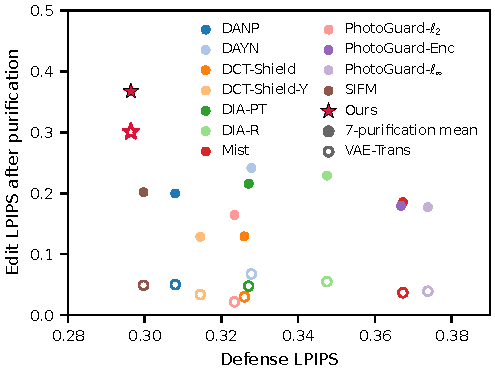
\includegraphics[width=\linewidth]{fig/purified_plane.pdf}
  \caption{Defense LPIPS versus edit LPIPS after purification at matched distortion on InstructPix2Pix (8 portraits $\times$ 4 instructions). Filled markers: mean over the seven standard purifications; open markers: after VAE-Trans.}
  \label{fig:purified_plane}
\end{figure}

\subsection{Without purification: one line for all methods}
\label{sec:exp_plane}
\Cref{fig:plane} plots edit displacement before purification against defense LPIPS for every method, including budget sweeps for six of them. The 34 points of the additive methods fit edit LPIPS $= 0.871 \times$ defense LPIPS $+ 0.072$ with $r = 0.955$, and each swept method stays on its own straight line ($r = 0.987$ to $1.000$). With DISTS or PieAPP on the horizontal axis, each method is still close to linear ($r = 0.87$ to $0.99$), but the slopes differ between methods. Our defense lies 0.044 above the pooled LPIPS line. Before purification, the color mapping and the additive methods are thus comparable at equal distortion. \Cref{tab:native} lists the methods at their native budgets, where defense LPIPS ranges from 0.043 to 0.666 and the ranking of displacement follows the ranking of distortion.

\begin{figure}[t]
  \centering
  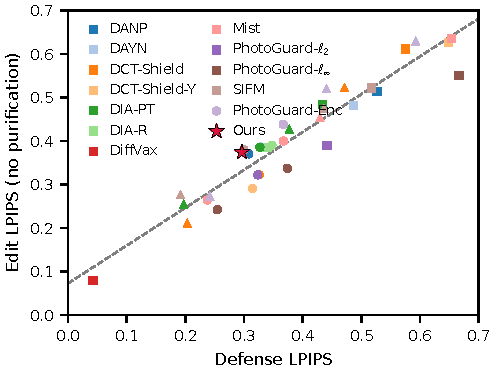
\includegraphics[width=\linewidth]{fig/plane.pdf}
  \caption{Defense LPIPS versus edit LPIPS before purification on InstructPix2Pix (8 portraits $\times$ 4 instructions). Squares: native budgets; circles: matched-distortion arm; triangles: budget sweeps. The dashed line is the least-squares fit to the 34 additive points ($r = 0.955$).}
  \label{fig:plane}
\end{figure}

\begin{table}[t]
  \centering
  \small
  \setlength{\tabcolsep}{3pt}
  \begin{tabular}{lccccc}
    \toprule
    & & \multicolumn{3}{c}{Edit LPIPS} & \\
    Method & Def. & None & 7-mean & Lowest & Ret. \\
    \midrule
    Mist & .654 & .636 & .503 & .379 & .793 \\
    PhotoGuard-$\ell_\infty$ & .666 & .551 & .461 & .322 & .843 \\
    DANP & .527 & .514 & .409 & .291 & .809 \\
    SIFM & .517 & .522 & .392 & .300 & .767 \\
    DCT-Shield-Y & .648 & .626 & .366 & .136 & .593 \\
    DAYN & .487 & .481 & .364 & .267 & .776 \\
    DIA-PT & .433 & .483 & .308 & .191 & .648 \\
    DCT-Shield & .575 & .611 & .261 & .131 & .435 \\
    PhotoGuard-$\ell_2$ & .442 & .390 & .255 & .123 & .658 \\
    DIA-R & .339 & .386 & .226 & .108 & .600 \\
    DiffVax & .043 & .079 & .081 & .065 & 1.059 \\
    \midrule
    Ours & .296 & .374 & .367 & .339 & 1.020 \\
    \bottomrule
  \end{tabular}
  \caption{Native budgets on InstructPix2Pix (8 portraits $\times$ 4 instructions). Def.: defense LPIPS; Ret.: retention over the seven purifications. Lowest is Gaussian blur $\sigma = 2$ except for DiffVax ($\sigma = 1$) and ours (crop-and-resize). PhotoGuard-Enc has no native-budget run.}
  \label{tab:native}
\end{table}

\subsection{What purification removes}
\label{sec:exp_purify}
To see what a purifier $P$ does to the defense itself, before any editing, we compute the fraction of the perturbation that survives, $\mathrm{LPIPS}(P(\tilde{x}), P(x)) / \mathrm{LPIPS}(\tilde{x}, x)$. \Cref{tab:survival} shows the result. Geometric operations (crop-resize, rotation) leave most perturbations in place for every method. JPEG, blur, and VAE purification are where the methods separate. Strong blur leaves 5--22\% of an additive perturbation and VAE purification leaves 2--9\%, while a LUT keeps most of its change because the colors of the photo survive these operations.

\begin{table}[t]
  \centering
  \small
  \setlength{\tabcolsep}{3.5pt}
  \begin{tabular}{lccccc}
    \toprule
    Method & Def. & 7-mean & JPEG30 & Blur2 & VAE \\
    \midrule
    DAYN & .328 & .535 & .398 & .219 & .092 \\
    DIA-R & .348 & .515 & .337 & .167 & .071 \\
    DANP & .308 & .483 & .317 & .167 & .070 \\
    DIA-PT & .327 & .473 & .295 & .130 & .059 \\
    SIFM & .300 & .467 & .303 & .143 & .053 \\
    PhotoGuard-$\ell_\infty$ & .374 & .387 & .205 & .088 & .034 \\
    Mist & .367 & .382 & .216 & .088 & .038 \\
    PhotoGuard-$\ell_2$ & .323 & .377 & .180 & .071 & .019 \\
    PhotoGuard-Enc & .367 & .373 & .202 & .101 & .039 \\
    DCT-Shield-Y & .315 & .312 & .209 & .057 & .038 \\
    DCT-Shield & .326 & .288 & .123 & .048 & .027 \\
    \midrule
    Penalty LUT (ablation) & .287 & .838 & .858 & .693 & .457 \\
    Ours & \NUM & \NUM & \NUM & \NUM & \NUM \\
    \bottomrule
  \end{tabular}
  \caption{Fraction of the perturbation that survives purification, $\mathrm{LPIPS}(P(\tilde{x}), P(x)) / \mathrm{LPIPS}(\tilde{x}, x)$, averaged over 8 images. Def.: defense LPIPS; 7-mean: mean over the seven standard purifications.}
  \label{tab:survival}
\end{table}

We then vary the strength of each purifier and edit the purified images (\cref{tab:strength}). For the additive methods, edit displacement falls steadily as JPEG quality drops or blur grows, reaching 0.03--0.14 at the strongest settings. For reference, editing the same undefended image with two different seeds already gives 0.109. The penalty-based LUT (ablation) stays between 0.25 and 0.34 over the whole range, and JPEG compression barely affects it.

\begin{table}[t]
  \centering
  \small
  \setlength{\tabcolsep}{3pt}
  \begin{tabular}{lcccccc}
    \toprule
    & \multicolumn{2}{c}{JPEG quality} & \multicolumn{2}{c}{Blur $\sigma$} & \multicolumn{2}{c}{Resize} \\
    Method & 95 & 10 & 0.5 & 3 & 0.75 & 0.25 \\
    \midrule
    DIA-PT & .336 & .135 & .334 & .044 & .277 & .108 \\
    Mist & .306 & .138 & .324 & .039 & .239 & .083 \\
    PhotoGuard-Enc & .289 & .129 & .311 & .040 & .221 & .086 \\
    DCT-Shield & .072 & .087 & .229 & .033 & .142 & .042 \\
    Penalty LUT (ablation) & .339 & .340 & .325 & .245 & .310 & .276 \\
    Ours & \NUM & \NUM & \NUM & \NUM & \NUM & \NUM \\
    \bottomrule
  \end{tabular}
  \caption{Edit displacement (LPIPS) after purification at increasing strength; 8 images $\times$ 4 instructions, InstructPix2Pix, matched distortion.}
  \label{tab:strength}
\end{table}

\TODO{Note on DCT-Shield, whose displacement is low already at JPEG quality 95 and does not decrease monotonically with strength.}

A matched random LUT also survives purification (0.196 after VAE-Trans), which tells us that the robustness comes from the carrier. Optimization adds the strength: within the same family, optimized mappings displace edits 32--61\% more than random ones at equal distortion.

\subsection{Other editors}
\label{sec:exp_gen}
InstructPix2Pix, SD inpainting, and SD 2.1 share the same VAE encoder weights, so a defense computed for one of them targets all three. On SD inpainting the penalty-based LUT gives 0.343 before purification, 0.288--0.323 under the seven purifications, and 0.241 after VAE-Trans, close to its InstructPix2Pix numbers. FLUX.1 Kontext~\cite{flux2025kontext} and UltraEdit~\cite{zhao2024ultraedit}, which builds on SD3, have their own 16-channel VAEs. Defenses computed on InstructPix2Pix and evaluated on these two editors keep the ranking of methods (Spearman 0.951). \TODO{Per-encoder results: ours optimized on the FLUX and SD3 encoders; baselines that can be ported with their own losses (PhotoGuard encoder attack, DCT-Shield, DCT-Shield-Y, and the textural term of Mist).}

\subsection{Is the result still a good photo?}
\label{sec:exp_percept}
Our defenses change the colors of the image on purpose, so we do not expect them to score well on metrics that compare against the original. They do not. PieAPP, TOPIQ-FR, AHIQ, CKDN, CW-SSIM, NLPD, GMSD, and MS-SSIM all rank the LUT defenses below the additive ones, and so do PickScore~\cite{kirstain2023pickscore} and HPSv3~\cite{ma2025hpsv3}. These numbers mix two things: the change of tone, which is intended and visible, and any damage to the image, which is not intended.

To separate them, we fit a global color transform from each defended image back to the original and measure what remains. With a smooth $9^3$ LUT as the transform, the penalty-based LUT drops from 0.287 to 0.137 LPIPS, below every additive method (0.282--0.358), and its DISTS, PieAPP, and SSIM fall inside the additive range. With a simpler affine transform in Lab, LPIPS drops to 0.209 but DISTS and PieAPP stay above the additive methods. Since aligning a LUT with a LUT may look circular, we apply the same alignment to twenty color-grading presets~\cite{rawtherapee_haldclut}. Film presets align almost perfectly (0.010--0.043), while some creative presets do not (bleach bypass stays at 0.340). Before alignment, the penalty-based LUT changes the image about as much as a creative preset (LPIPS 0.287 against 0.061--0.353) and more than a film preset (0.031--0.115).

No-reference scores tell a similar story. Relative to the original, the LAION aesthetic score of the penalty-based LUT rises by 0.175 (additive methods: $-0.061$ to $+0.145$), and MUSIQ, CLIP-IQA, and ImageReward fall by amounts inside the additive range. \TODO{User study: two-alternative naturalness judgments and edited-or-not detection following~\cite{scooter2025}; final numbers for our method.}

\subsection{Ablations}
\label{sec:exp_ablation}
\Cref{tab:ablation} lists the ablations. The first row compares ways of keeping the mapping natural, from per-artifact penalties solved with an augmented Lagrangian to the rotation parameterization of \cref{sec:feasible}.

\begin{table}[t]
  \centering
  \small
  \setlength{\tabcolsep}{3pt}
  \begin{tabular}{ll}
    \toprule
    Axis & Variants \\
    \midrule
    Naturalness & per-artifact penalties / single-constant bounds / feasible set / rotation (ours) \\
    Rotation & single angle bound / separate saturation and hue bounds \\
    Carrier & RGB curves / $(a^*, b^*)$ warp / LUT $17^3$, $33^3$ \\
    Objective & encoder latent / equivariance / implicit classifier \\
    Control & random LUT and random filter, matched distortion \\
    \bottomrule
  \end{tabular}
  \caption{Ablation axes. \TODO{numbers}}
  \label{tab:ablation}
\end{table}
